\documentclass{beamer}

\mode<presentation> {
	\usetheme{Antibes}
	\setbeamertemplate{footline}[page number]	
	\setbeamertemplate{navigation symbols}{}
	\setbeamertemplate{items}[square]
}

\usepackage{graphicx}
\usepackage{booktabs}
\usepackage{hyperref}

\newcommand{\link}[2]{\href{#1}{\textit{\color{blue}{#2}}}}%


\title[DragonFly]{Project DragonFly: Vehicle Surveillance System}
\institute[GCEK-CSE]{Department of Computer Science and Engineering \\Government College of Engineering Kannur}
\author[Group 3]{
	{\small \textit{Guided by:}} Dr. Rafeeque P.C \\
	\medskip
	{\small \textbf{\textit{Group 3}}} \\
	Abhinand C \\ Edwin Jose George \\ Lavanya E.V \\ Shilpa Suresh
}
\date{\today}

%Results
%Result -Analysis( Use graphs/ metric relevent to your work )
%Conclusion
%Future Scope
%References


% result analysis
% challange and future emprovemtns

\begin{document}
	
	%---------------------------------------------------------------------------
	% METADATA -----------------------------------------------------------------
	%---------------------------------------------------------------------------

	\begin{frame}
	\titlepage
	\end{frame}

	\begin{frame}{Table of Contents}
	\tableofcontents
	\end{frame}


	%---------------------------------------------------------------------------
	% INTRODUCTION -------------------------------------------------------------
	%---------------------------------------------------------------------------

	\section{Introduction}
	\subsection{Motivation}
	\begin{frame}{Motivation}		
		Policing agencies have setup vast networks of distributed surveillance cameras along major routes. The sheer amount of data generated is overwhelming for manual analysis, to trace routes of rouge vehicles.\\~\\
		
		Current system make use of manual approach of reviewing long video
		clips to identify the suspect vehicle. Various possible routes that can
		be taken by suspect further makes the process of re-identification very
		difficult and time consuming.\\~\\
				
		DragonFly is an AI based project that aims to resolve this particular issue. 
	\end{frame}

	\subsection{Objective}
	\begin{frame}{Objective}
		\begin{itemize}
			\item Aid in traffic policing by extracting and detecting various vehicle
			description
			\item Generate route map for a specific vehicle description, along with
			timestamps
			\item Conduct traffic analysis to predict traffic flow with existing sensor
			network.
			\item System is to be used by general public, which accounts for
			unstructured input of vehicle description.
		\end{itemize}
	\end{frame}

	\subsection{Literature Review}
	\begin{frame}{Literature Review}
		\begin{table}[!h]
			\centering
			\resizebox{\textwidth}{!}{%
				\begin{tabular}{|l|l|l|l|}
					\hline
					\multicolumn{1}{|c|}{\textit{\textbf{Title}}} &
					\multicolumn{1}{c|}{\textit{\textbf{Method}}} &
					\multicolumn{1}{c|}{\textit{\textbf{Pros and Cons}}} &
					\multicolumn{1}{c|}{\textit{\textbf{Challenges}}} \\ \hline
					\begin{tabular}[c]{@{}l@{}}CityFlow: A City-Scale \\ Benchmark for Multi-Target\\ Multi-Camera  Vehicle\\  Tracking and  \\ Re-Identification\end{tabular} &
					\begin{tabular}[c]{@{}l@{}}Use of Multi-Target Single Camera\\ and Multi-Target Multi-Camera \\ tracking.\\ \\ Use visual-spatio-temporal\\ reasoning\end{tabular} &
					\begin{tabular}[c]{@{}l@{}}Pros:\\ Better and faster results.,\\ Handle large scale recognition\\ Tracking and small prediction\\ \\ Cons:\\ Overlapping viewpoints,\\ Implemented only at junction \\ points\end{tabular} &
					\begin{tabular}[c]{@{}l@{}}High quality videos\\ \\ Multiple viewpoints on \\ same object\\ \\ Require annotated videos\end{tabular} \\ \hline
					\begin{tabular}[c]{@{}l@{}}Real-Time Vehicle Make and\\ Model Recognition System\end{tabular} &
					\begin{tabular}[c]{@{}l@{}}Random Forest and Support Vector\\  Machine coupled with traditional\\ Vehicle Make Model Recognition\\ System,\\ \\ Usage of Histogram of Oriented \\ Gradient (HOG) and GIST \\ features\end{tabular} &
					\begin{tabular}[c]{@{}l@{}}Pros:\\ Superior processing speed \& \\ recognition accuracy wrt existing \\ VMMR, Accounts for partial \\ viewpoints\\ \\ Cons:\\ High dimensional,  Region of \\ interest is only on parts, No global\\  representation\end{tabular} &
					\begin{tabular}[c]{@{}l@{}}Computational time increases\\ with increase of blocks HOG\\ \\ Limited Region of Interest\end{tabular} \\ \hline
					\begin{tabular}[c]{@{}l@{}}Efficient and Deep Vehicle \\ Re-Identification Using \\ Multi-Level Feature \\ Extraction\end{tabular} &
					\begin{tabular}[c]{@{}l@{}}Global channel extracts single \\ feature generalizing whole image,\\ \\ Local channel extract multiple\\  local features (logo, stickers),\\ \\ Attribute channel extracts \\ color, model, type\end{tabular} &
					\begin{tabular}[c]{@{}l@{}}Pros:\\ Extraction of inter and intra features,\\ Data augmentation with license plate \\ verification\\ \\ Cons:\\ Requires Data augmentation,\\ Effected by illuminations\end{tabular} &
					\begin{tabular}[c]{@{}l@{}}Cross camera vehicle tracking\\ \\ Changes in color response\\ \\ Background clutter\end{tabular} \\ \hline
				\end{tabular}%
			}
		\end{table}
		% include NVIDIA AI challange, papers regarding yolov4, paddlepaddle, github repository
	\end{frame}

	\subsection{Problem Statement}
	\begin{frame}{Problem Statement}
		A novel approach to provide an integrated platform utilizing existing infrastructure to monitor transport sector, and extend timely information to policing agencies, with intuitive interface.
	\end{frame}

	\begin{frame}{Contributions}
		\begin{itemize}
			\item Custom YOLOv4 AI model trained on Indian vehicles
			\item Integration of various AI based algorithm and models (YOLOv4, deepSORT, siamese Network)
			\item Simple user interface supporting elastic search
			\item Optimization of back-end services that are containerized 
		\end{itemize}
	\end{frame}
	
	
	%---------------------------------------------------------------------------
	% DESIGN AND IMPLEMENTATION ------------------------------------------------
	%---------------------------------------------------------------------------	
	
	\section{Design and Implementation}
	\begin{frame}{Proposed System}
		\begin{itemize}
			\item The user provides the system with vehicle descriptions such as color, model, location, time-period etc. 
			\item The system finds corresponding match by making use of various AI techniques. 
			\item The system tries to re-identify the said vehicle across multiple camera locations.
			\item The system finds the path followed by the said vehicle along with the detected frame at each camera points.
		\end{itemize}
	\end{frame}

	\begin{frame}{Algorithm}
		\framesubtitle{Dummy camera network}
		\begin{center}
			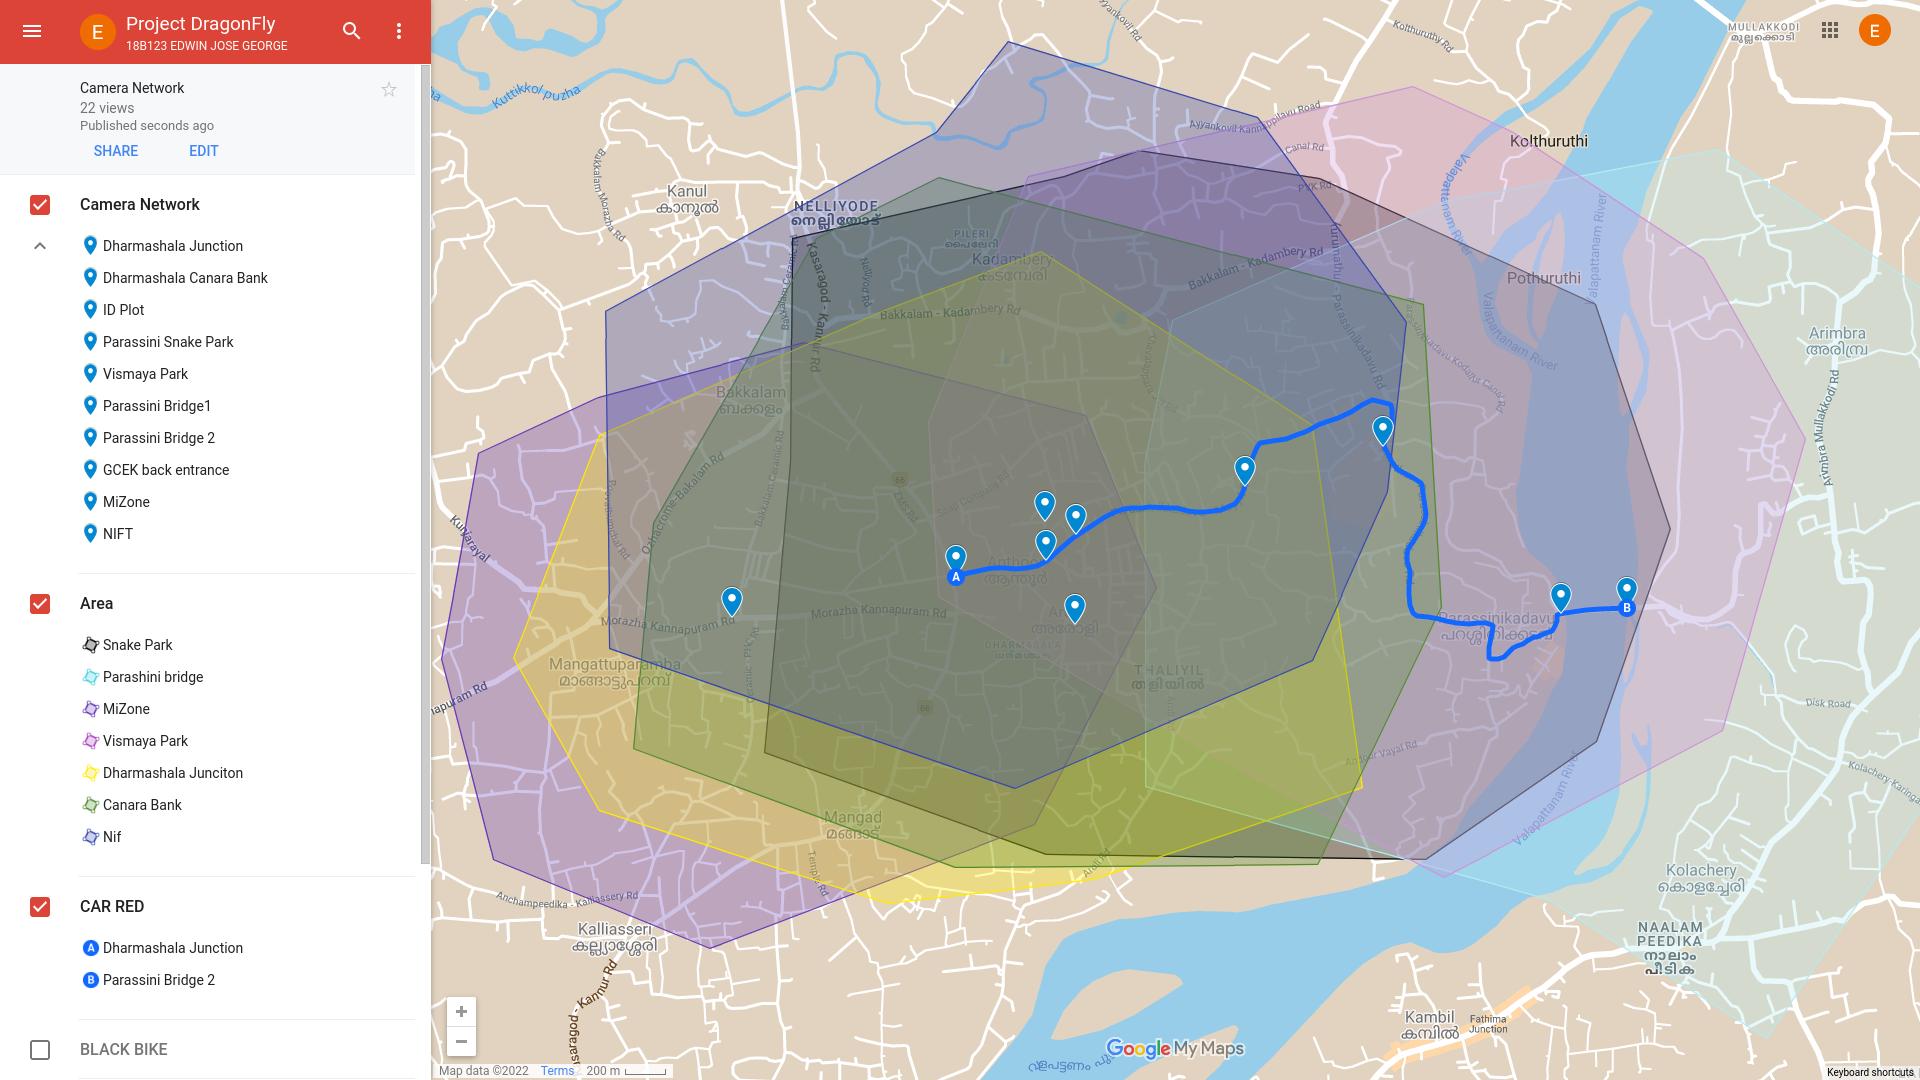
\includegraphics[height=0.7\textheight]{res/camera_network_demo.png}
		\end{center}
		Created with \link{https://www.google.com/maps/d/edit?mid=1s2ST5x4nn-EK3JqU-c9EEGASRq5Ini0&usp=sharing}{Google Maps}
	\end{frame}
	
	\subsection{System Architecture}
	\begin{frame}{Architecture Design}
		\begin{center}
			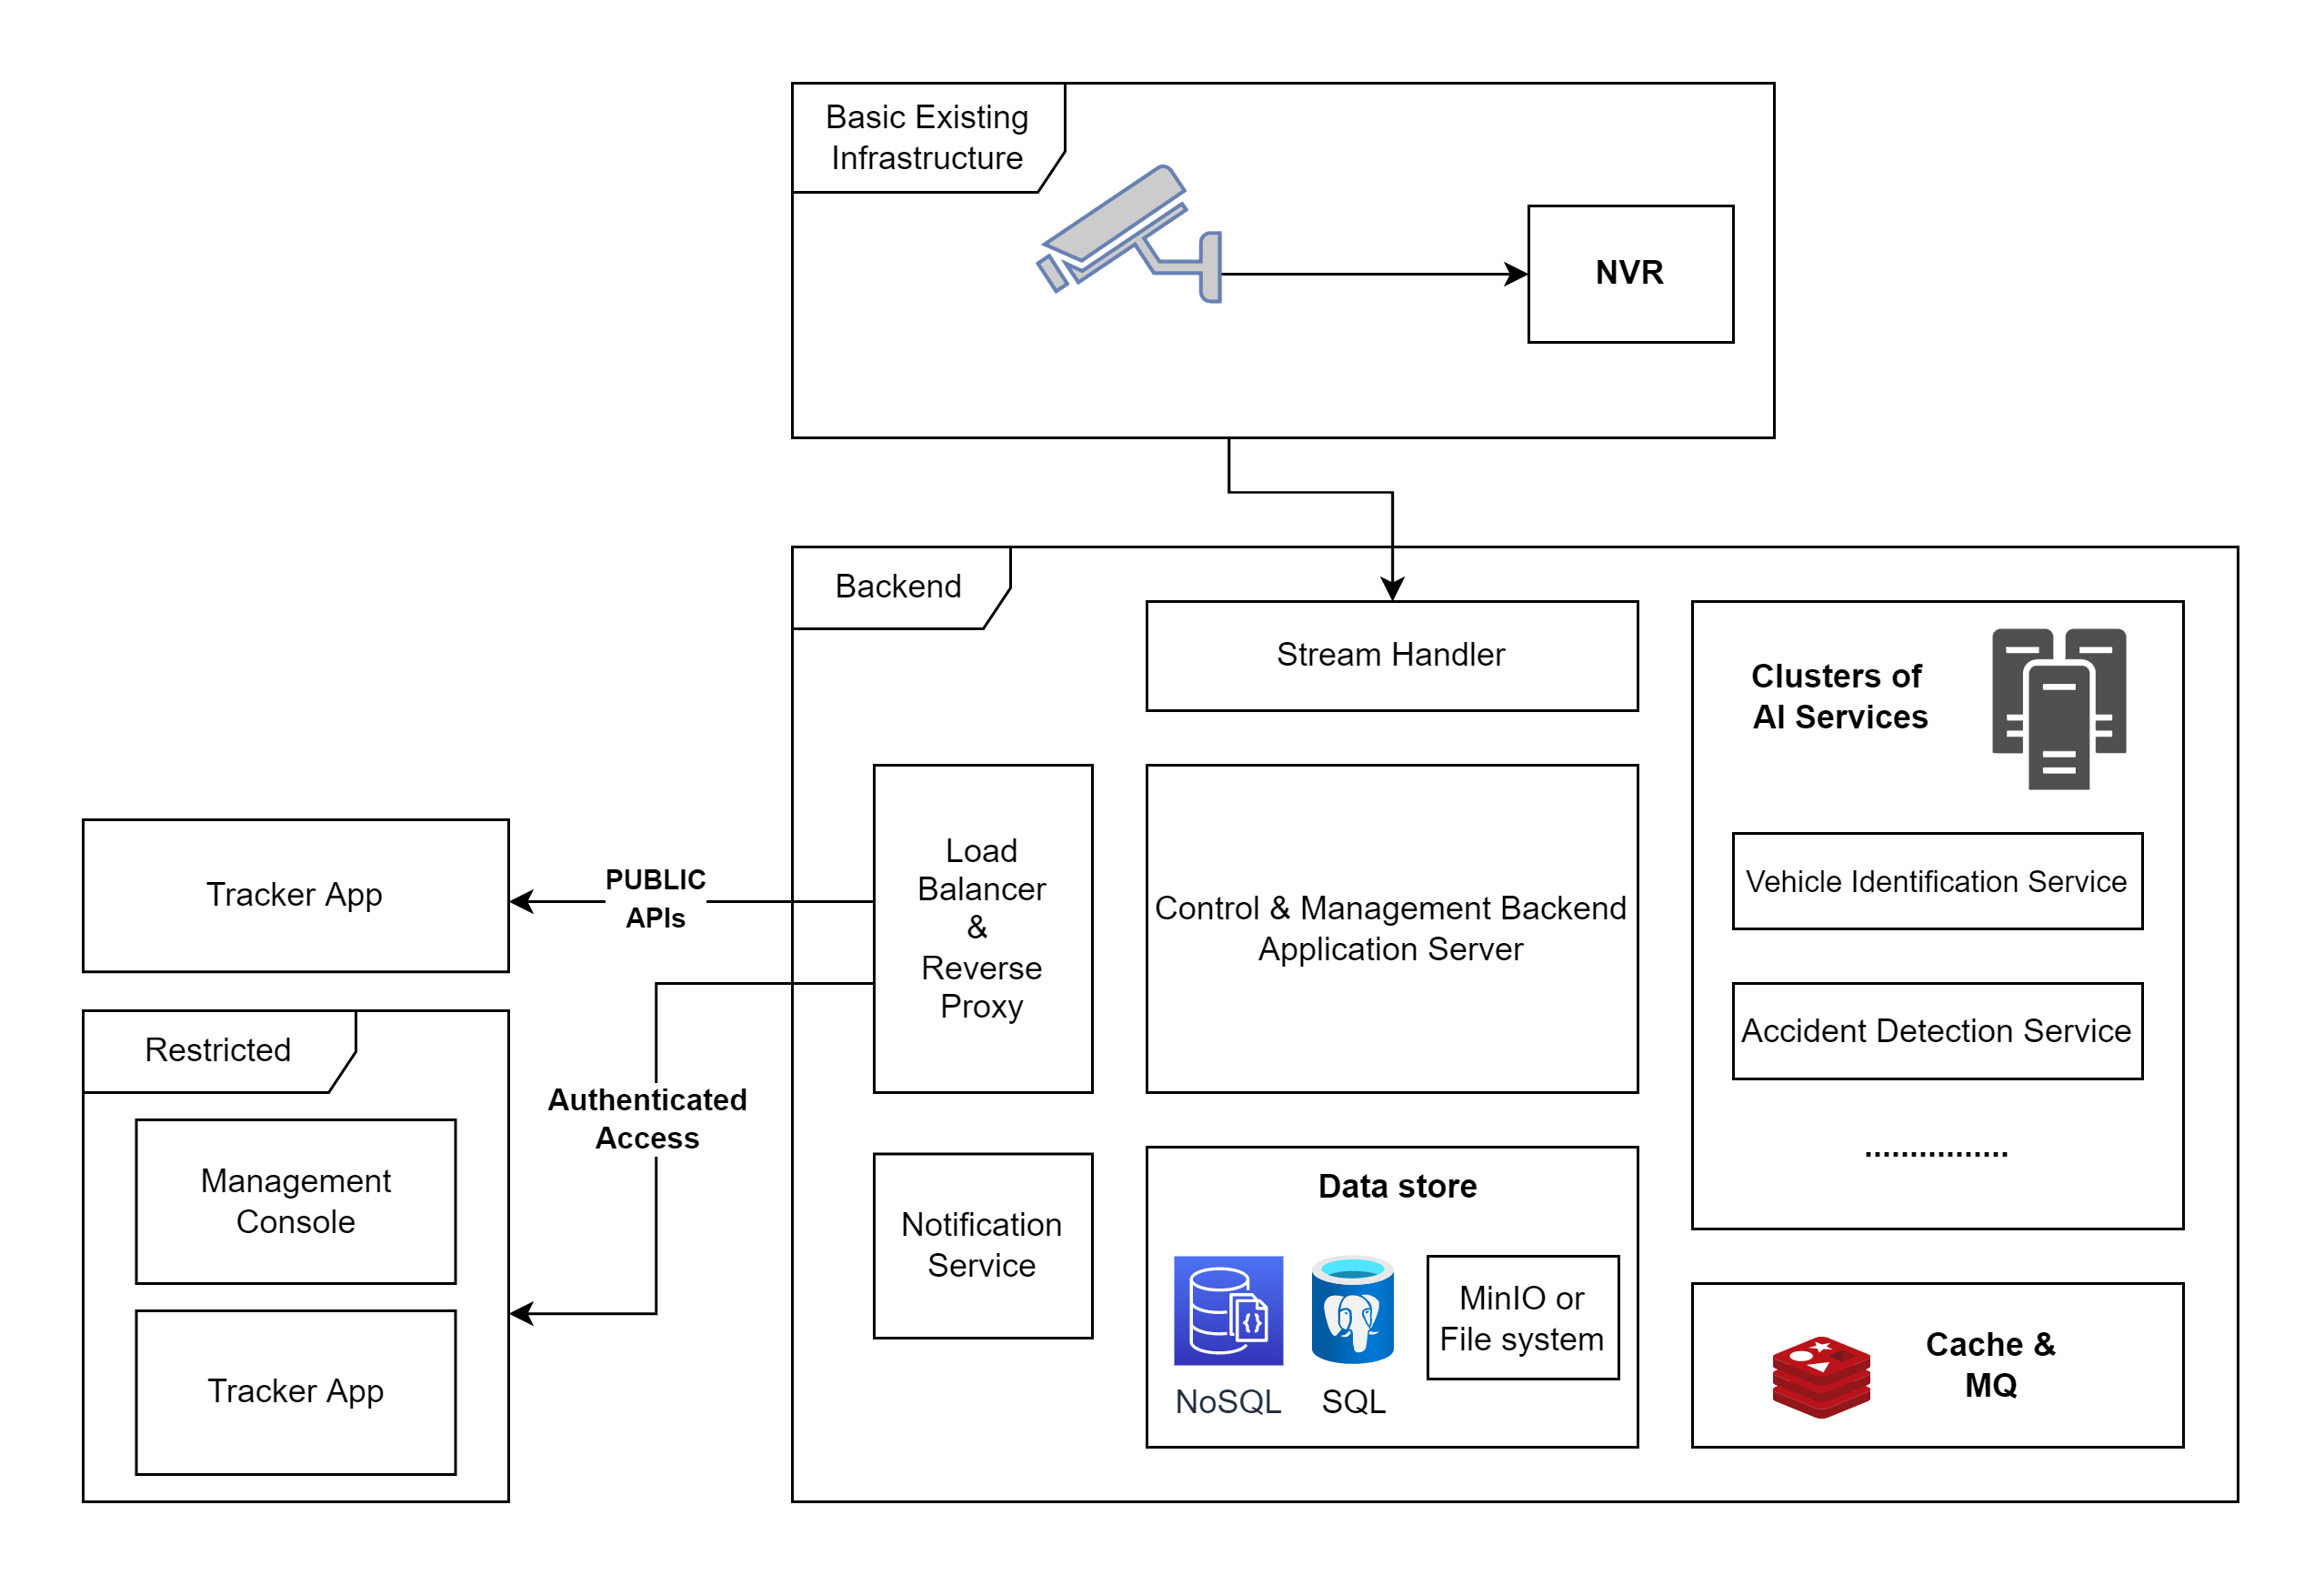
\includegraphics[width=\linewidth]{res/architecture_high_level}
		\end{center}
	\end{frame}

	\begin{frame}{Pipeline1}
		\begin{center}
			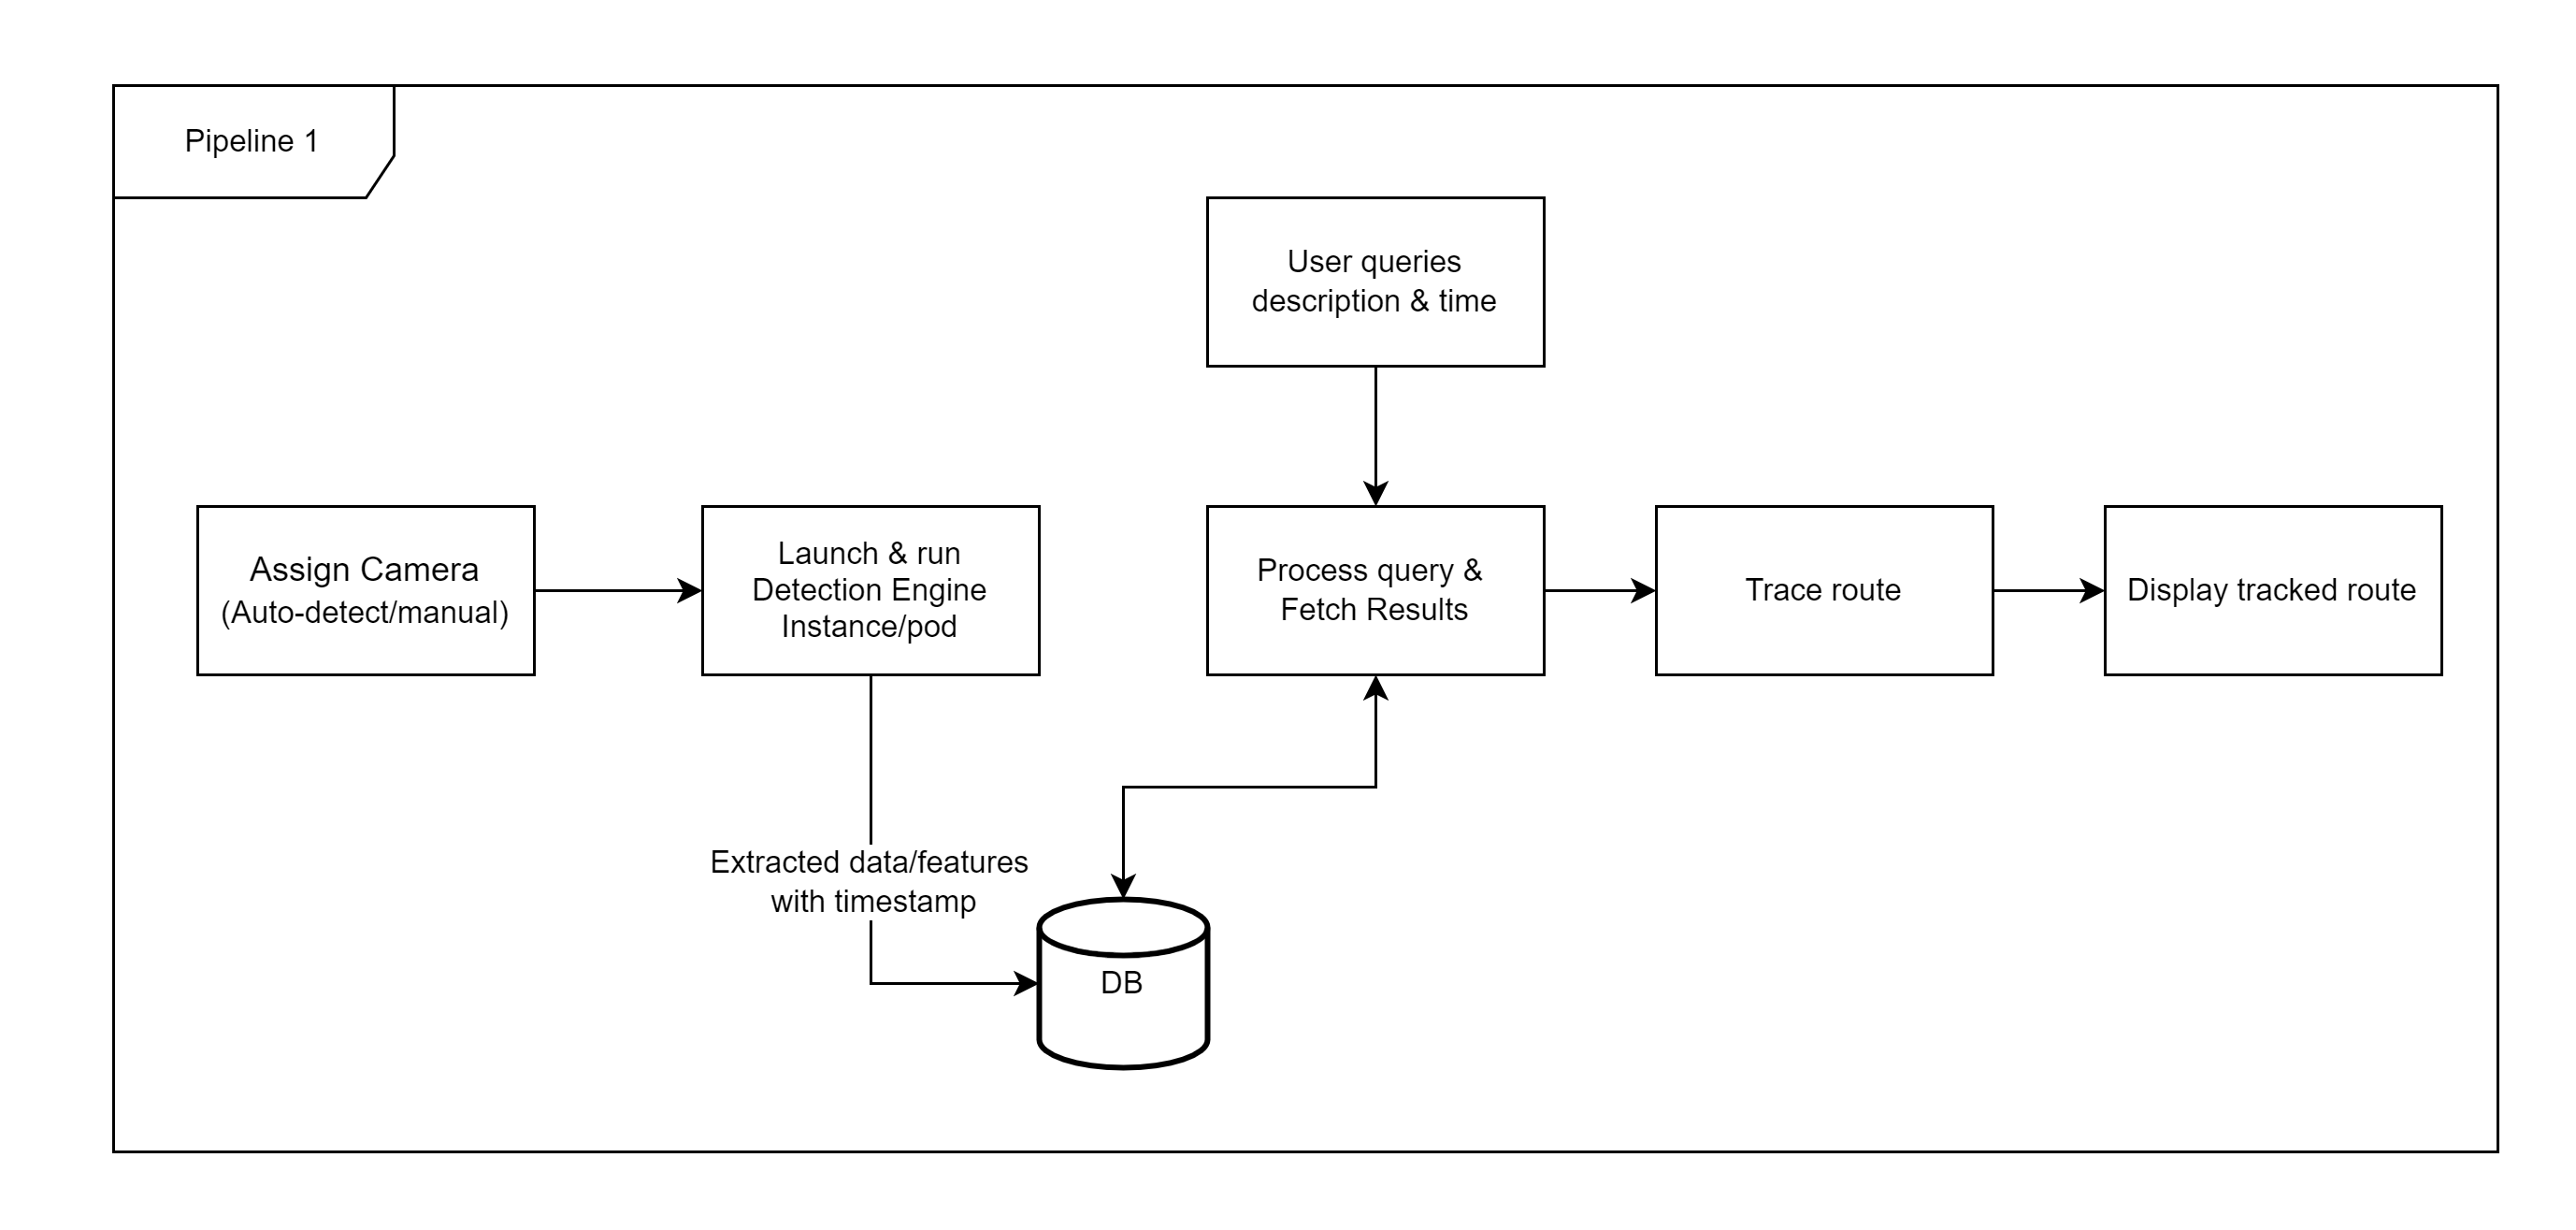
\includegraphics[width=\linewidth]{res/pipeline1}
		\end{center}
	\end{frame}

	\begin{frame}{Pipeline2}
		\begin{center}
			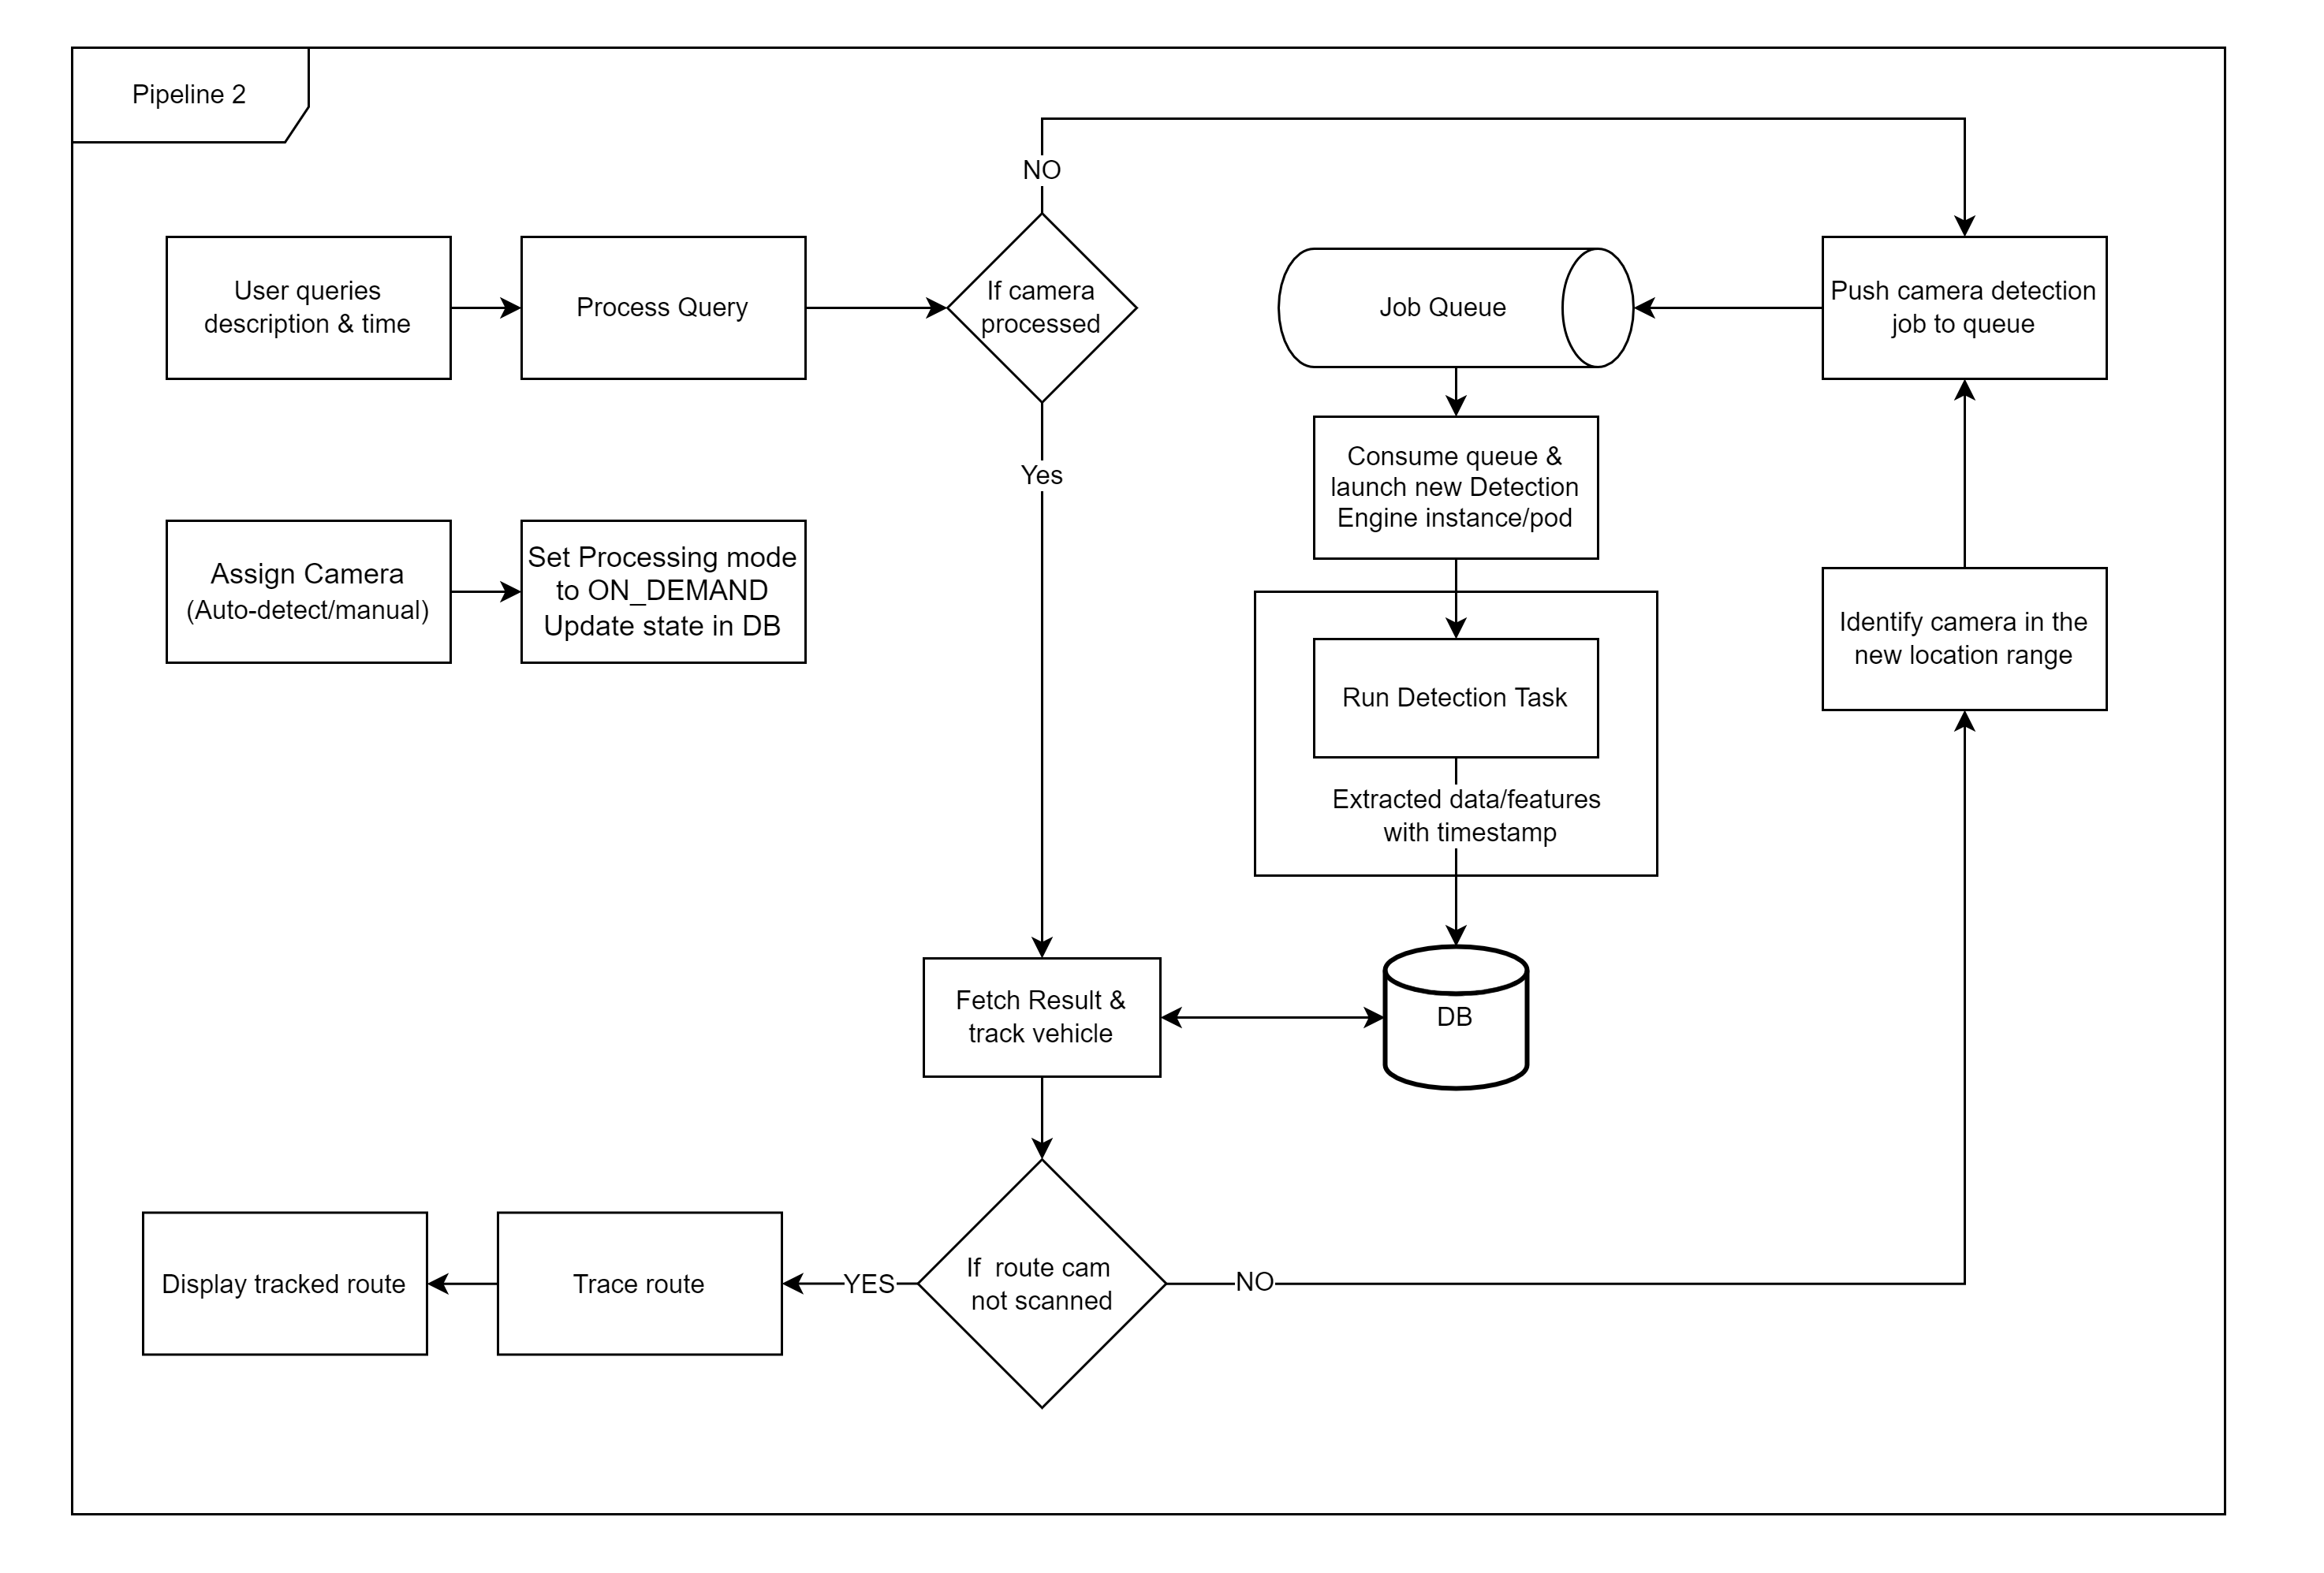
\includegraphics[width=\linewidth]{res/pipeline2}
		\end{center}
	\end{frame}

	\subsection{AI Models}
	\begin{frame}{YOLOv4}
		\framesubtitle{Architecture}
		\begin{center}
			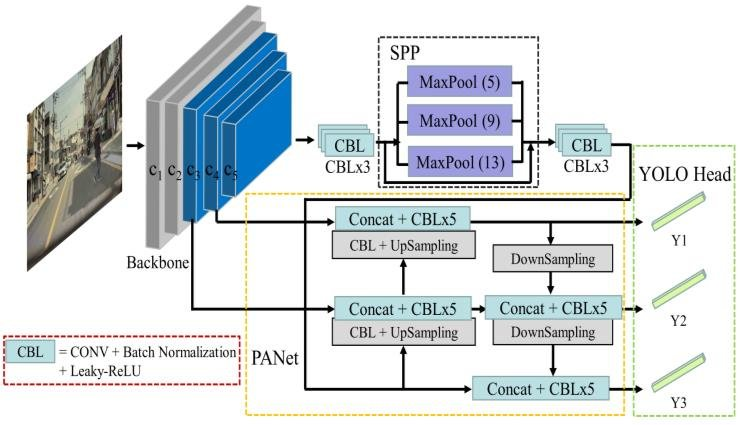
\includegraphics[width=0.8\linewidth]{res/YOLOV4-research-gate.png}
		\end{center}
		Image imported from \link{https://www.researchgate.net/figure/Overall-structure-of-YOLOv4-including-CSPDarknet-backbone-SPPnet-PANet-and-3-YOLO\_fig2\_344919620}{researchgate}. Find the implemented model architecture from \link{https://github.com/Project-Dragon-Fly/Dragon-Fly-Slides/blob/main/final-implementation-review/res/yolov4-vehicle.svg}{here}.
	\end{frame}

	\begin{frame}{YOLOv4}		
		\framesubtitle{Model Parameters}
		\begin{table}[]
			\centering
			\resizebox{\textwidth}{!}{%
				\begin{tabular}{|l|l|}
					\hline
					Input size            & 416 * 416                    \\ \hline
					Input Channels            & 3   \\ \hline
					Batch size             & 32                          \\ \hline
					learning rate    & 0.0013 \\ \hline								Final input to yolo layer        & [256*256],[512*512],[1024*1024]                       \\ \hline
					Total Layers               & 162                     \\ \hline
					
					Target Classes & \begin{tabular}[c]{@{}l@{}}
						auto, bus, tempo traveler, tractor, \\
						truck, van, two wheeler, car, jcb\end{tabular} \\ \hline
				\end{tabular}%
			}
		\end{table}
	\end{frame}

	\begin{frame}{YOLOv4}		
		\framesubtitle{Model Training}
		\begin{table}[]
			\centering
			\resizebox{\textwidth}{!}{%
				\begin{tabular}{|l|l|}
					\hline
					Framework used            & DarkNet                    \\ \hline
					Initial weight            & official 80 class weight   \\ \hline
					Target classes            & 9                          \\ \hline
					Platform for training     & Google Colab + Workstation \\ \hline
					Current mAP               & 98.4 \%                    \\ \hline
					Current Iterations        & 7300                       \\ \hline
					DataSet & \begin{tabular}[c]{@{}l@{}}500 till 2800 iteration\\ 733 after wards\end{tabular} \\ \hline
					Approx Hrs Spent training & 35-48 hrs                \\ \hline
				\end{tabular}%
			}
		\end{table}
	\end{frame}

	\begin{frame}[allowframebreaks]{Dataset - Kaggle}
		Fetched from \link{https://www.kaggle.com/datasets/dataclusterlabs/indian-vehicle-dataset}{Kaggle}. Used labelImg to label images. 
		\begin{table}[]
			\centering
			\begin{tabular}{|l|l|}
				\hline
				\textbf{Frequency}    & \textbf{Label Name} \\ \hline
				557                   & two wheeler         \\ \hline
				354                   & truck               \\ \hline
				297                   & auto                \\ \hline
				233                   & car                 \\ \hline
				220                   & bus                 \\ \hline
				133                   & tractor             \\ \hline
				101                   & van                 \\ \hline
				1                     & jcb                 \\ \hline
				\textbf{Total Boxes}  & \textbf{1956}       \\ \hline
				\textbf{Total Images} & \textbf{733}        \\ \hline
			\end{tabular}
		\end{table}
		
		
		
		\newpage
		\begin{figure}
			\includegraphics[width=0.24\linewidth]{"res/data_set1/image1"} \hfill
			\includegraphics[width=0.24\linewidth]{"res/data_set1/image2"} \hfill
			\includegraphics[width=0.24\linewidth]{"res/data_set1/image3"} \hfill
			\includegraphics[width=0.24\linewidth]{"res/data_set1/image4"}
		\end{figure}
	\end{frame}
	
	
	\begin{frame}[allowframebreaks]{Dataset - Camera Network}
		Fetched from camera infrastructure. Used labelImg to label images.
		\begin{center}
			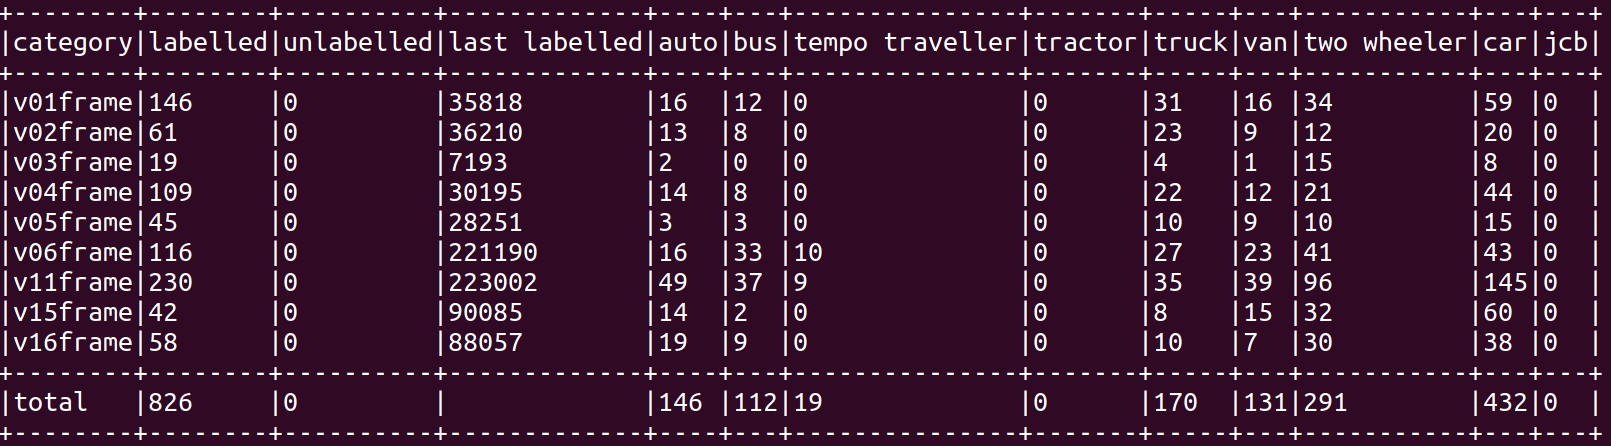
\includegraphics[width=\linewidth]{res/data_set2/custom_label_stat}
		\end{center}
		
		\newpage
		\begin{figure}
			\includegraphics[width=0.48\linewidth]{"res/data_set2/image1"} \hfill
			\includegraphics[width=0.48\linewidth]{"res/data_set2/image2"}
			\\[\smallskipamount]
			\includegraphics[width=0.48\linewidth]{"res/data_set2/image3"} \hfill
			\includegraphics[width=0.48\linewidth]{"res/data_set2/image4"}
		\end{figure}
	\end{frame}


	\begin{frame}{deepSORT}
		\begin{center}
			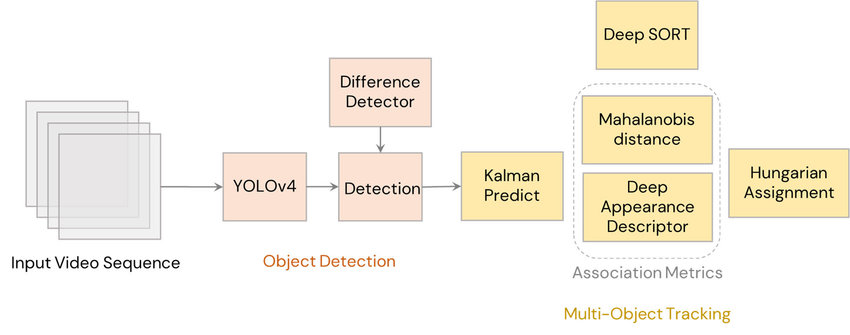
\includegraphics[width=0.95\linewidth]{res/deepSORT.png}
		\end{center}
		Image imported from \link{https://www.researchgate.net/figure/Architecture-of-Deep-SORT-Simple-online-and-real-time-tracking-with-deep-association\_fig2\_353256407}{researchgate}.
	\end{frame}

	\begin{frame}{Siamese Network}
		\begin{center}
			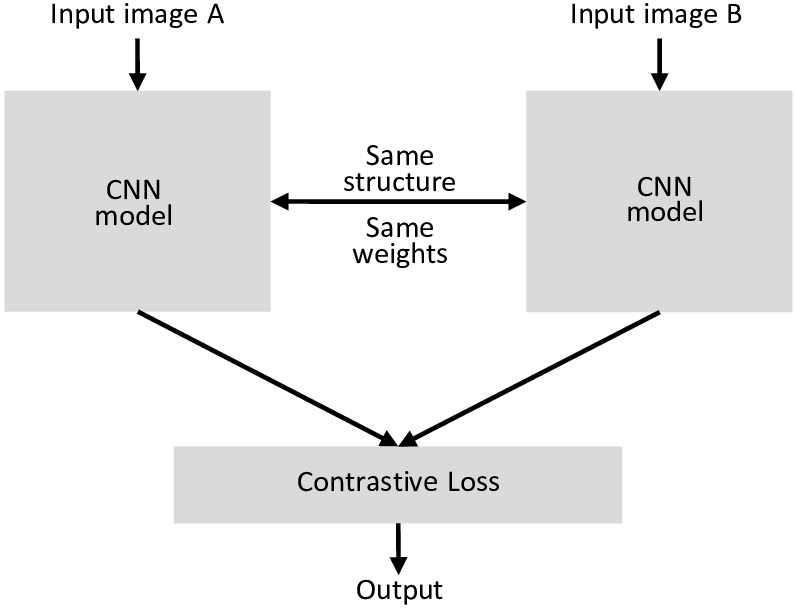
\includegraphics[height=0.6\textheight]{res/siamese-network.png}
		\end{center}
		Image imported from \link{https://www.researchgate.net/figure/Structure-of-the-Siamese-network\_fig1\_327494280}{researchgate}.
	\end{frame}


	\subsection{UI Design}
	\begin{frame}{Vehicle Image Dictionary}
		\begin{center}
			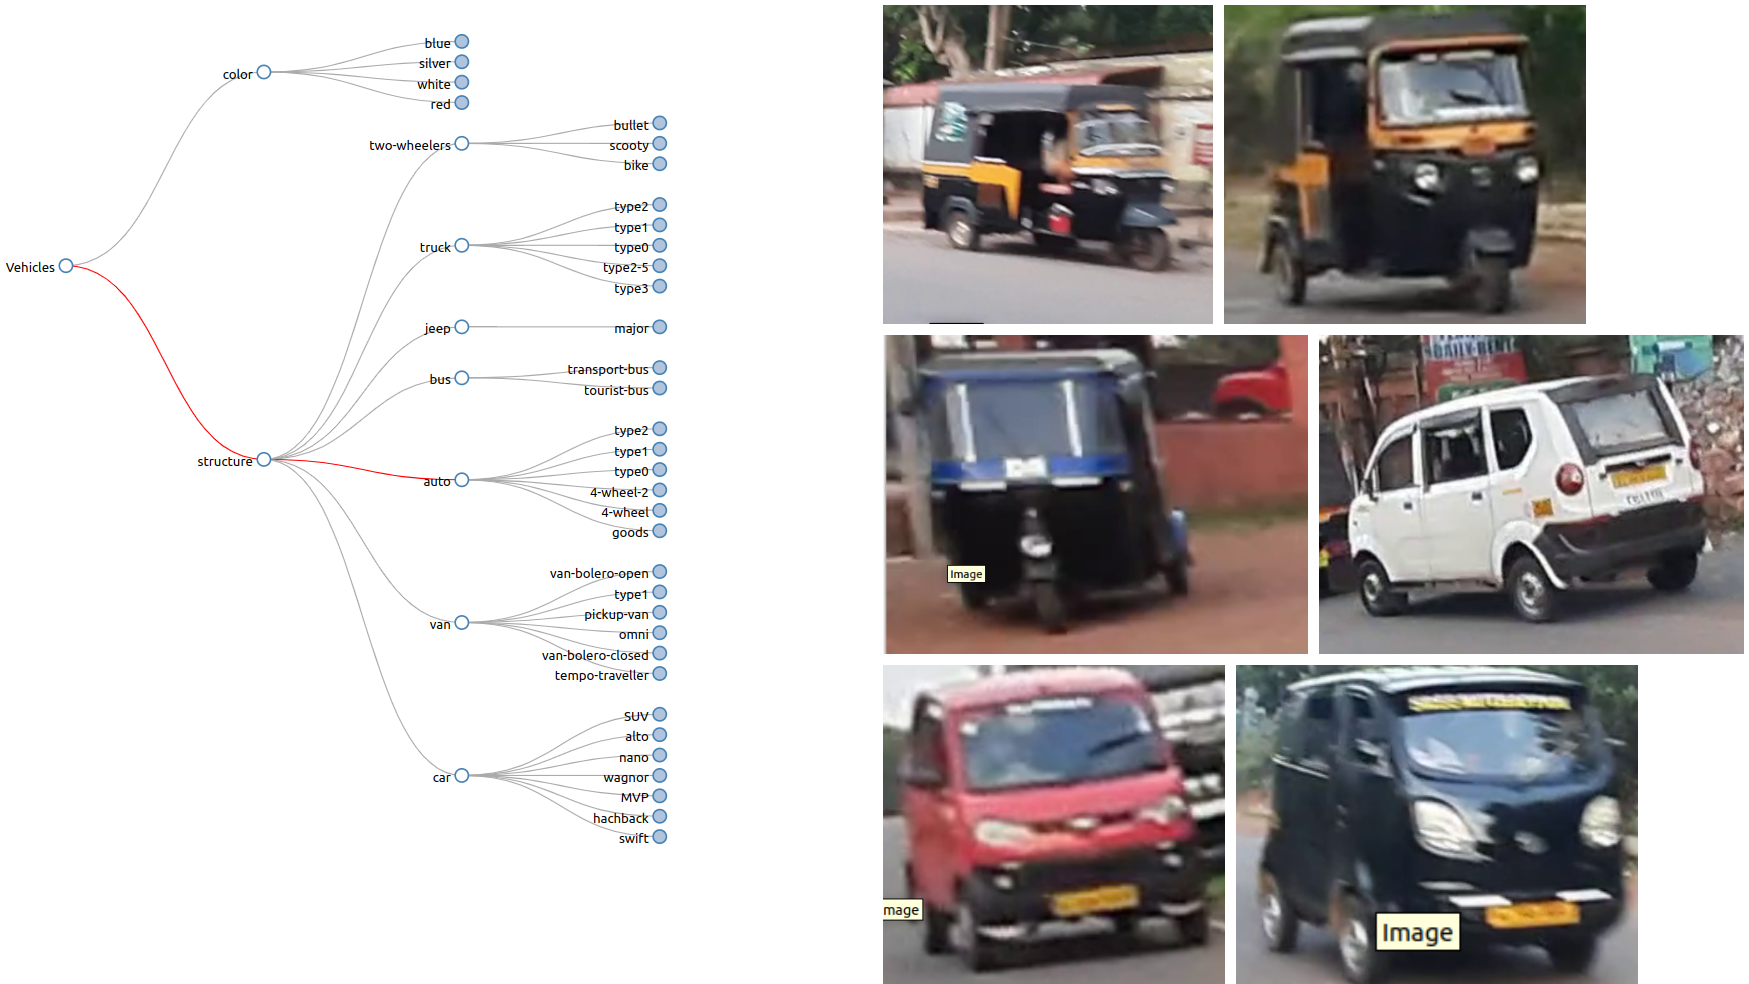
\includegraphics[width=\linewidth]{res/image_dictionary.png}
		\end{center}
	\end{frame}

	\begin{frame}{Login Page}
		\begin{center}
			% \includegraphics[width=\linewidth]{res/image.png}
		\end{center}
 	\end{frame}
 
	 \begin{frame}{Tracking Vehicle}
	 	\begin{center}
	 		% \includegraphics[width=\linewidth]{res/image.png}
	 	\end{center}
	 \end{frame}
 
	 \begin{frame}{Building Route Map}
		\begin{center}
			% \includegraphics[width=\linewidth]{res/image.png}
		\end{center}
	\end{frame}

	

	
	


	%---------------------------------------------------------------------------
	% RESULTS ------------------------------------------------------------------
	%---------------------------------------------------------------------------

	\section{Results}
	\subsection{AI model}
	\begin{frame}{YOLOv4 model}
		\framesubtitle{Training - Loss and Accuracy chart}
		\begin{center}
			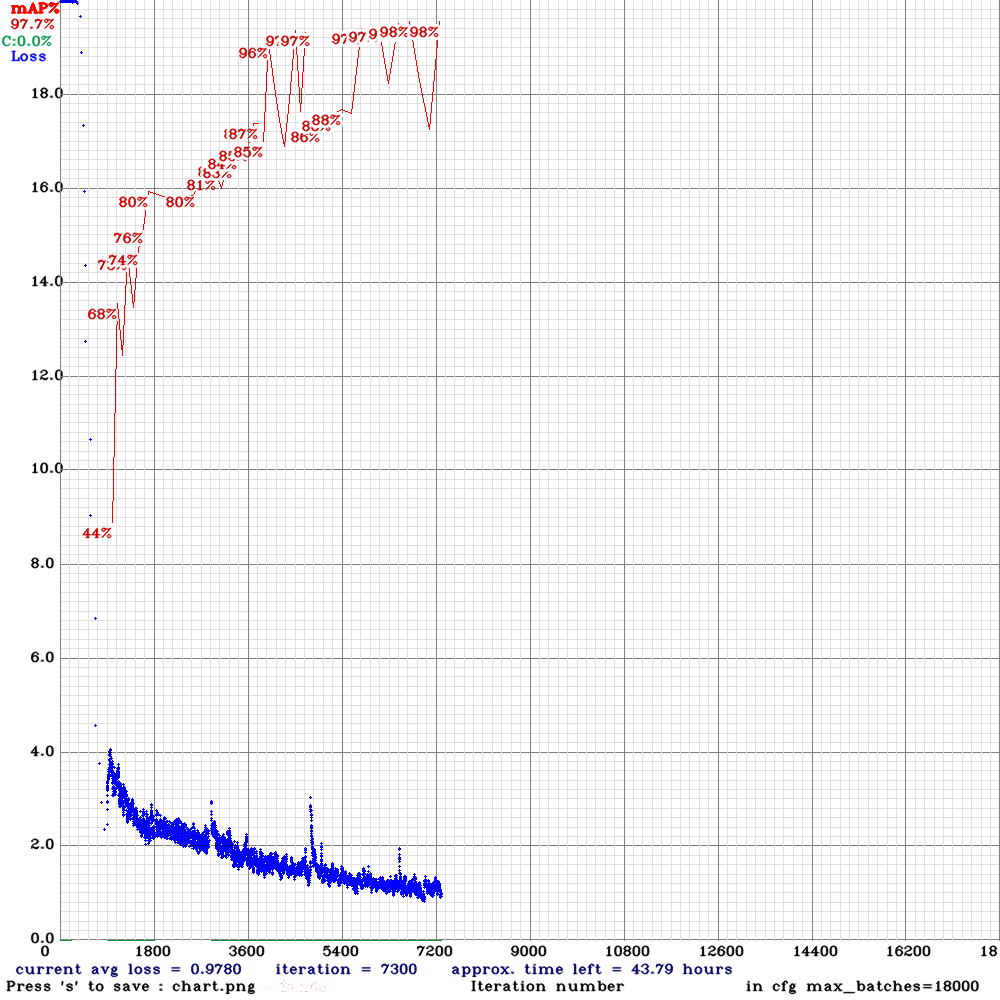
\includegraphics[height=0.7\textheight]{res/darknet_training_chart}
		\end{center}
	\end{frame}

	\begin{frame}{YOLOv4 model}
		\framesubtitle{Accuracy}
		\begin{scriptsize}
			detections\_count = 7729, unique\_truth\_count = 1956  \\ 
			class\_id = 0, name = auto, ap = 97.27\%   	 (TP = 285, FP = 15) \\
			class\_id = 1, name = bus, ap = 99.76\%   	 (TP = 217, FP = 10) \\
			class\_id = 2, name = tempo traveller, ap = 96.50\%   	 (TP = 57, FP = 3) \\
			class\_id = 3, name = tractor, ap = 98.93\%   	 (TP = 131, FP = 1) \\
			class\_id = 4, name = truck, ap = 99.20\%   	 (TP = 346, FP = 36) \\
			class\_id = 5, name = van, ap = 96.71\%   	 (TP = 98, FP = 21) \\
			class\_id = 6, name = two wheeler, ap = 88.59\%   	 (TP = 480, FP = 104) \\
			class\_id = 7, name = car, ap = 93.92\%   	 (TP = 216, FP = 39) \\
			class\_id = 8, name = jcb, ap = 100.00\%   	 (TP = 0, FP = 0) \\
			
			for conf\_thresh = 0.25, precision = 0.89, recall = 0.94, F1-score = 0.91  \\
			for conf\_thresh = 0.25, TP = 1830, FP = 229, FN = 126, average IoU = 72.94 \%  \
			
			IoU threshold = 50 \%, used Area-Under-Curve for each unique Recall  \\
			mean average precision (mAP@0.50) = 0.967638, or 96.76 \% \\
			Total Detection Time: 268 Seconds
		\end{scriptsize}		
	\end{frame}

	\begin{frame}{YOLOv4 model}
		\framesubtitle{Prediction}
		\begin{center}
			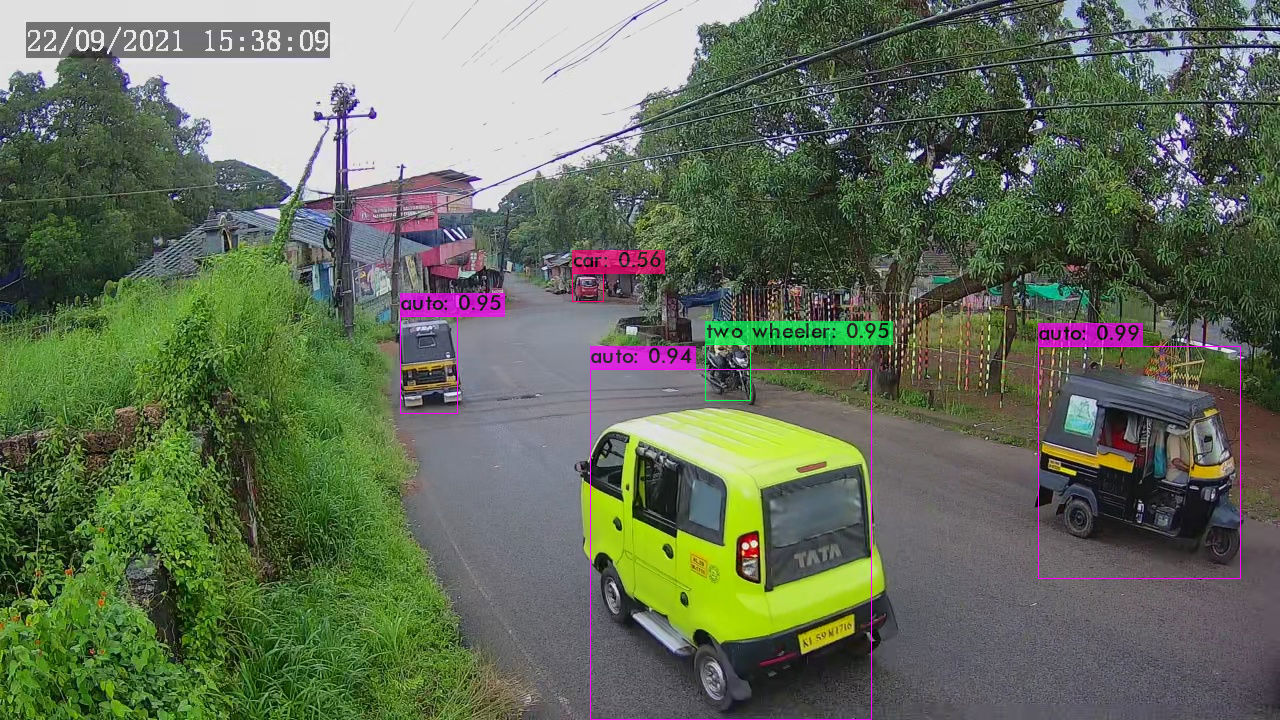
\includegraphics[width=\linewidth]{res/data_set1/predictions}
		\end{center}
	\end{frame}



	\subsection{UI/UX}	
	\begin{frame}{Login page}
		\begin{center}
			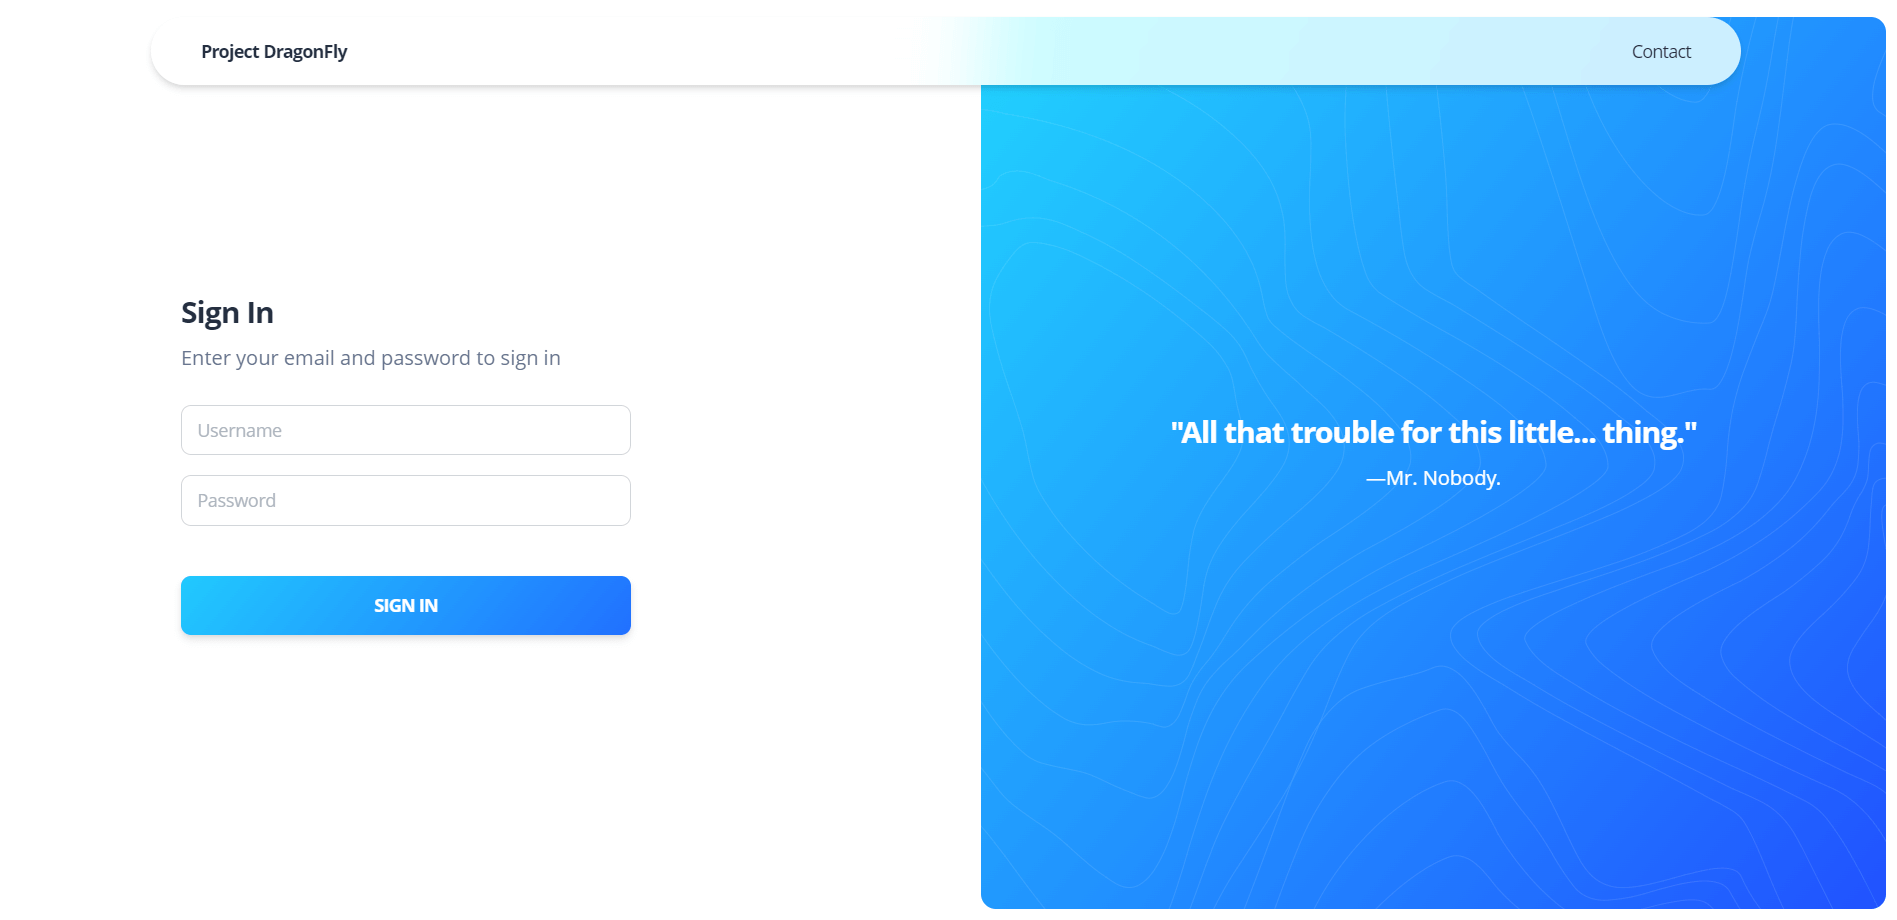
\includegraphics[width=1\linewidth]{res/loginpage.png}
		\end{center}
	\end{frame}

	\begin{frame}{Home page}
		\begin{center}
			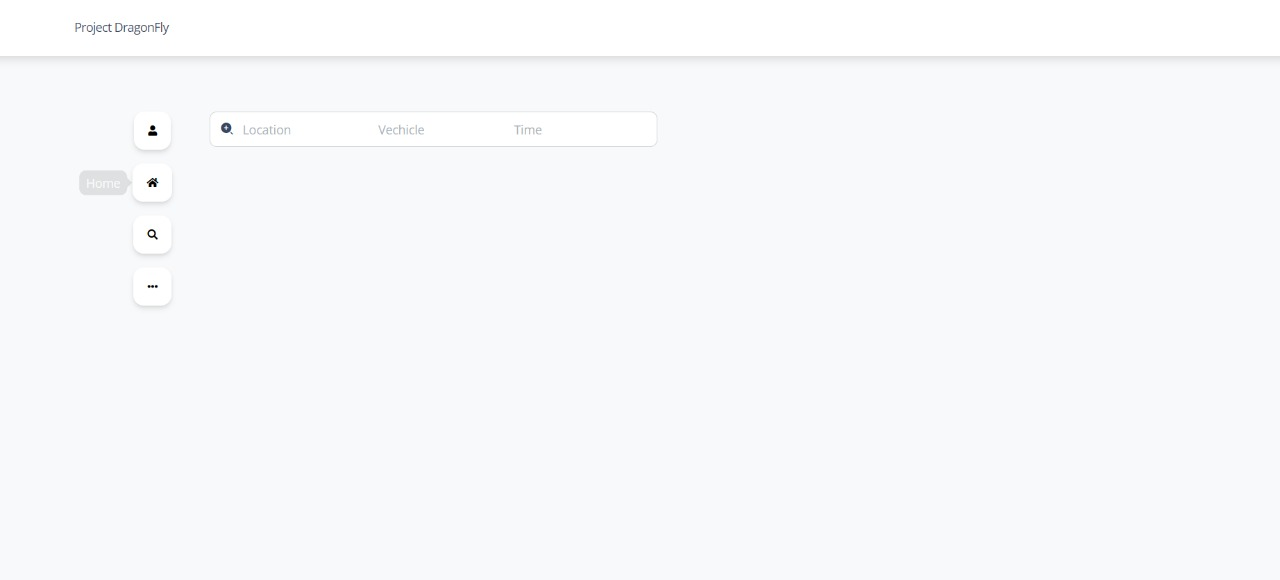
\includegraphics[width=1\linewidth]{res/homepage}
		\end{center}
	\end{frame}

	\begin{frame}{Result Page}
		\begin{center}
			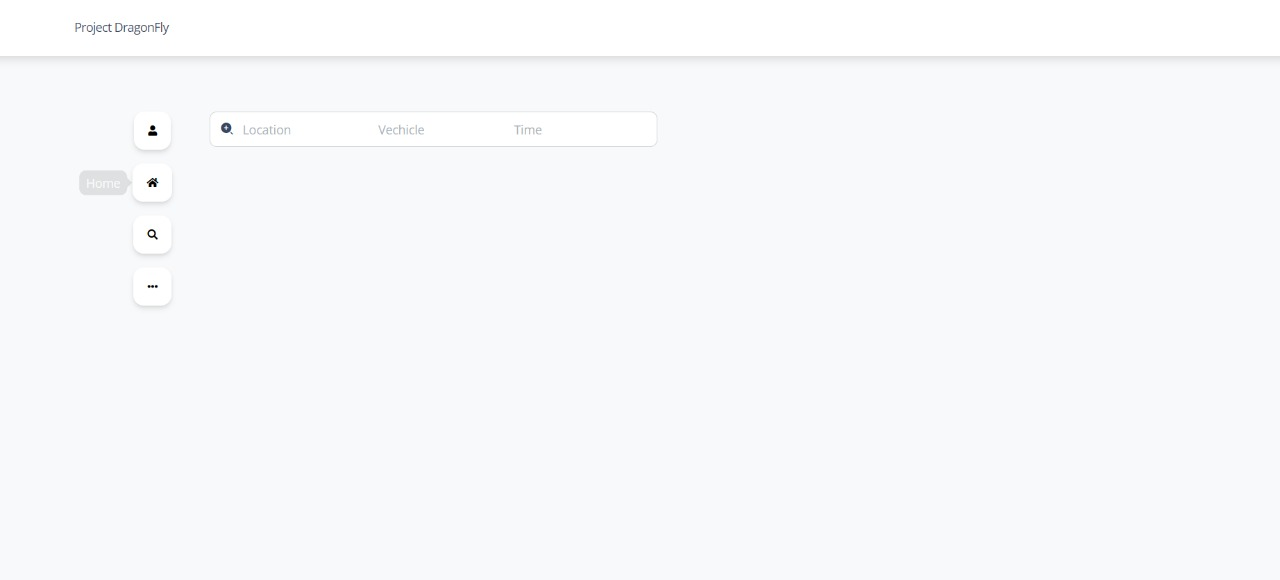
\includegraphics[width=1\linewidth]{res/homepage}
		\end{center}
	\end{frame}

%	\subsection{Other Updates}
%	\begin{frame}{Works done : Other updates}
%		\begin{itemize}
%			\item Defining service communication data format - laying structures \link{https://github.com/Project-Dragon-Fly/mock-servers/blob/main/data\_format.md}{visit here}
%			\item Development of \link{https://github.com/Project-Dragon-Fly/backend-server}{backend service} and \link{https://github.com/Project-Dragon-Fly/mock-servers}{mock servers}
%			\item Database design and simple route business logic 
%			\item Registered and acquired data from \link{https://www.aicitychallenge.org/}{NVIDIA AI City Challenge}
%			\item Obtained camera access and checked streaming data from video frames.
%			\item Exploring Google Maps API and Geo-Pandas.
%		\end{itemize}
%		\begin{center}
%			\link{https://github.com/Project-Dragon-Fly}{GitHub Organization} $|$ \link{https://drive.google.
%				com/drive/folders/1GbQ1L1mfY97nh3NXE4Iyz\_e2gIwvmH0V?usp=sharing}{Shared Google Drive}
%		\end{center}
%	\end{frame}

	\section{Result and Analysis}
	\begin{frame}[allowframebreaks, noframenumbering]{Results}
		
	\end{frame}


\section{References}
\begin{frame}[allowframebreaks, noframenumbering]{References}
	\nocite{*}
	\bibliographystyle{IEEEtran}
	\bibliography{IEEEabrv,reference.bib}
\end{frame}

\end{document} 